\documentclass[12pt]{beamer}
\usetheme{CambridgeUS}
\usepackage[utf8]{inputenc}
\usepackage[spanish]{babel}
\usepackage{amsmath}
\usepackage{amsfonts}
\usepackage{amssymb}
\usepackage{graphicx}
\author{Kevin Garcia - Alejandro Vargas}
\title{Modelo de regresión lineal múltiple}
%\setbeamercovered{transparent} 
%\setbeamertemplate{navigation symbols}{} 
%\logo{} 
%\institute{} 
%\date{} 
%\subject{} 
\begin{document}

\begin{frame}
\titlepage
\end{frame}

%\begin{frame}
%\tableofcontents
%\end{frame}
\begin{frame}
\frametitle{Definición de variables}
\begin{itemize}
\item Valor mediano de las viviendas:Se define como el valor medio que tiene una casa dentro del bloque.
\item Ingreso mediano:Siendo el ingreso una trasformación definimos el ingreso mediano como la cantidad mediana de dinero anual que entra a una vivienda dentro del bloque.
\item Edad mediana de las viviendas:Corresponde a la edad que tiene una vivienda dentro del bloque.
\item Total de habitaciones:Corresponde al total del numero de habitaciones que hay en una vivienda dentro de un bloque.
\item Total de dormitorios:Corresponde al total del numero de dormitorios que hay en una vivienda dentro de un bloque
\item Población:Corresponde al numero total de habitantes dentro de un bloque.
\item Hogares:Corresponde al total de familias que se auto denominan como unidad y habitan en una misma vivienda.
\item Latitud y longitud:Medidas de localización donde se encuentra cada bloque.
\end{itemize}
\end{frame}

\begin{frame}
\frametitle{Análisis exploratorio de datos}
~\\ Para trabajar con la base de datos denominada 'cadata', generamos un número aleatorio con la ayuda del software R, el cuál nos arrojó el número 15529, por tanto nuestra base de datos final, quedo con las 9 variables (columnas) y con las filas desde la 15529 hasta la 16028.

~\\ El objetivo del estudio es ajustar un modelo de regresión para la variable 'Valor mediano de las casas', tomando como variables explicativas las variables 'Ingreso mediano','Edad mediana de la vivienda', 'Total de habitaciones','Total de dormitorios','Población' y 'Hogares'. 
\end{frame}

\begin{frame}
\frametitle{Análisis exploratorio de datos}
~\\ Previo al ajuste e interpretación del modelo, se llevo a cabo el respectivo análisis exploratorio de datos, para tener una idea de las descriptivas mas importantes de cada variable, su forma de distribución y su rango de valores.
\end{frame}

\begin{frame}
\frametitle{Análisis exploratorio de datos}
\begin{figure}[!h]
    \begin{center}
        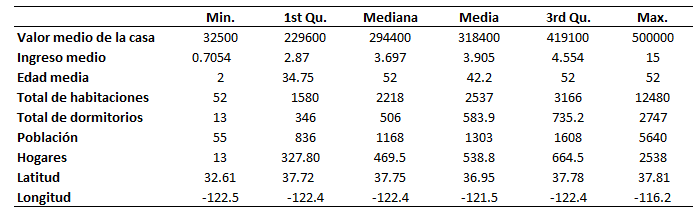
\includegraphics[width=12cm]{imagenes/estadisticas.png}
        \caption{Resumen estadístico}
        \label{fig:Densidad}
    \end{center}
\end{figure}

\end{frame}
\begin{frame}
\frametitle{Variable 'Valor mediano de las viviendas'}
\begin{figure}[!h]
    \begin{center}
        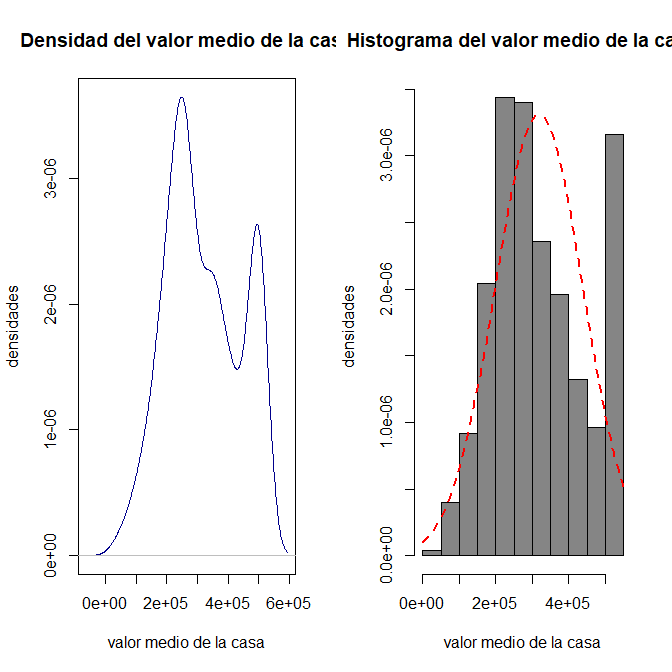
\includegraphics[width=11cm]{imagenes/1.png}
        \caption{Histograma y densidad de la variable 'Valor mediano de las casas'}
        \label{fig:Densidad}
    \end{center}
\end{figure}
\end{frame}
\begin{frame}
\frametitle{Variable 'Valor mediano de las viviendas'}
\begin{figure}[!h]
    \begin{center}
        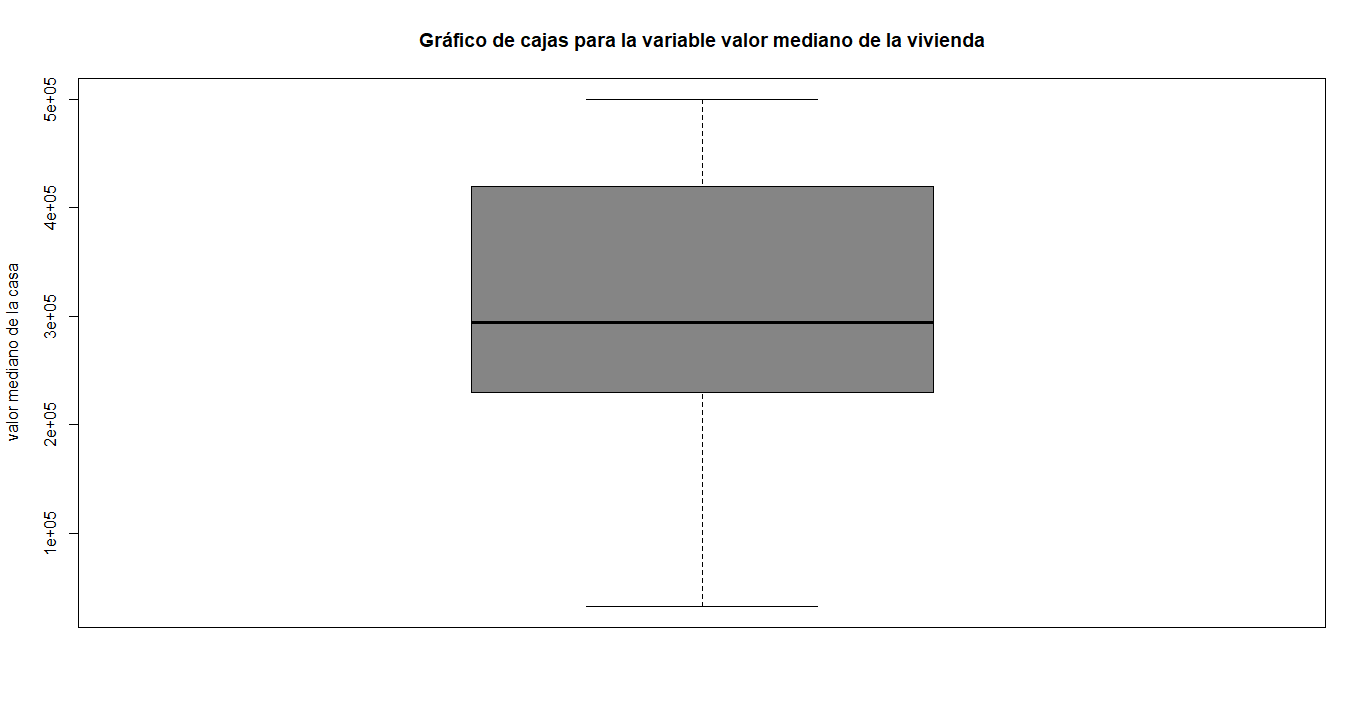
\includegraphics[width=11cm]{imagenes/12.png}
        \caption{Gráfico de cajas para la variable 'Valor mediano de las casas'}
        \label{fig:Densidad}
    \end{center}
\end{figure}
\end{frame}

\begin{frame}
\frametitle{Variable 'Ingreso mediano'}
\begin{figure}[!h]
    \begin{center}
        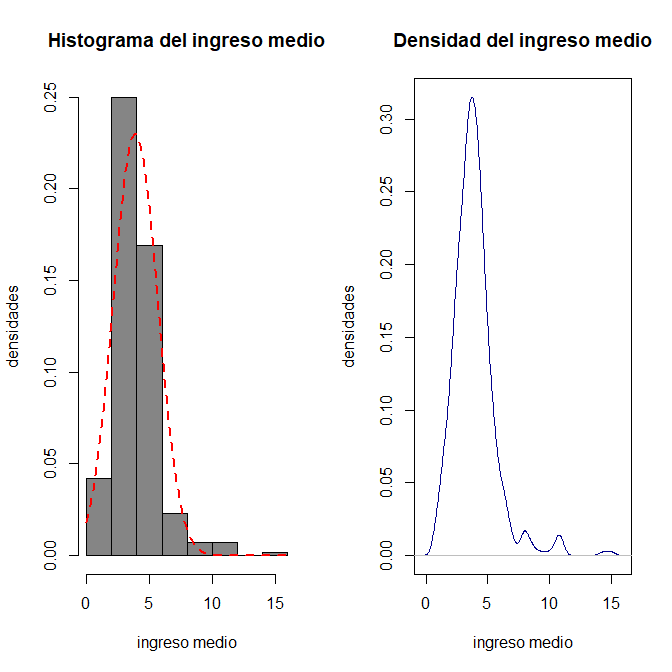
\includegraphics[width=11cm]{imagenes/2.png}
        \caption{Histograma y densidad de la variable 'Ingreso mediano'}
        \label{fig:Densidad}
    \end{center}
\end{figure}
\end{frame}
\begin{frame}
\frametitle{Variable 'Ingreso mediano'}
\begin{figure}[!h]
    \begin{center}
        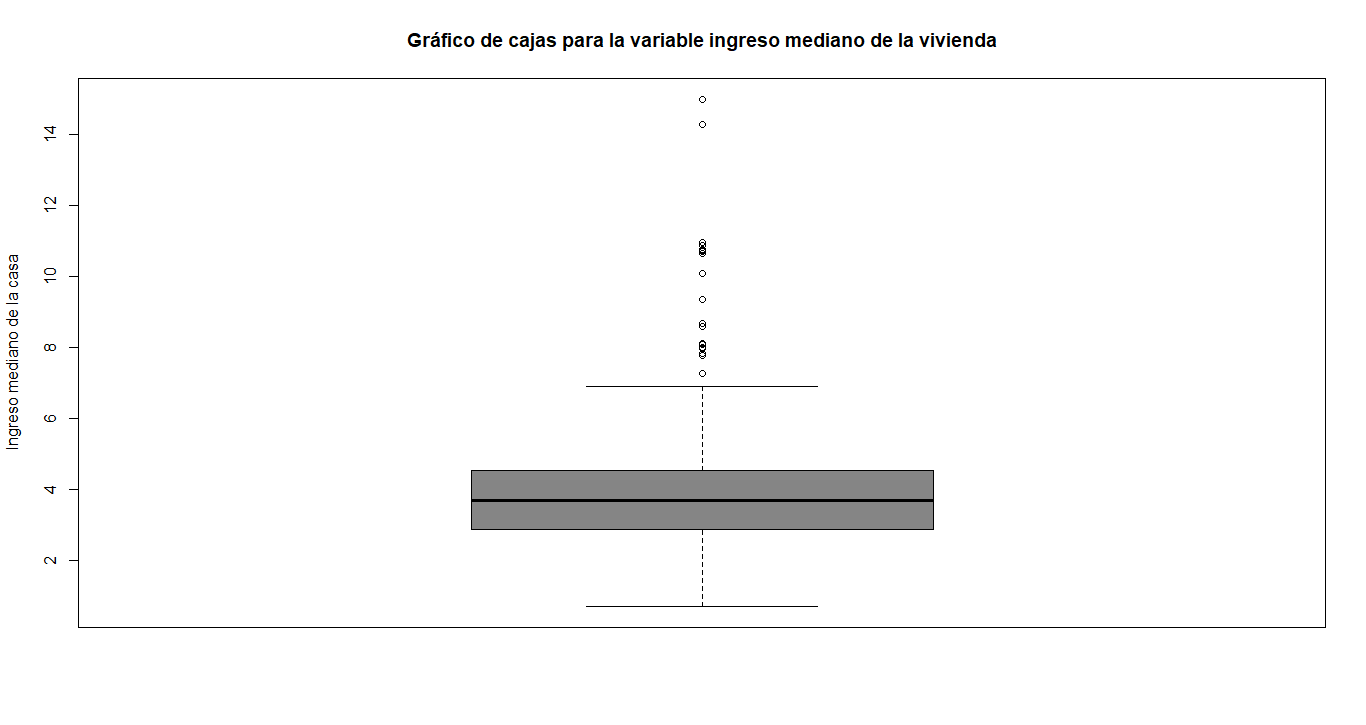
\includegraphics[width=11cm]{imagenes/13.png}
        \caption{Gráfico de cajas para la variable 'Ingreso mediano de las casas'}
        \label{fig:Densidad}
    \end{center}
\end{figure}
\end{frame}

\begin{frame}
\frametitle{Variable 'Edad mediana de las viviendas'}
\begin{figure}[!h]
    \begin{center}
        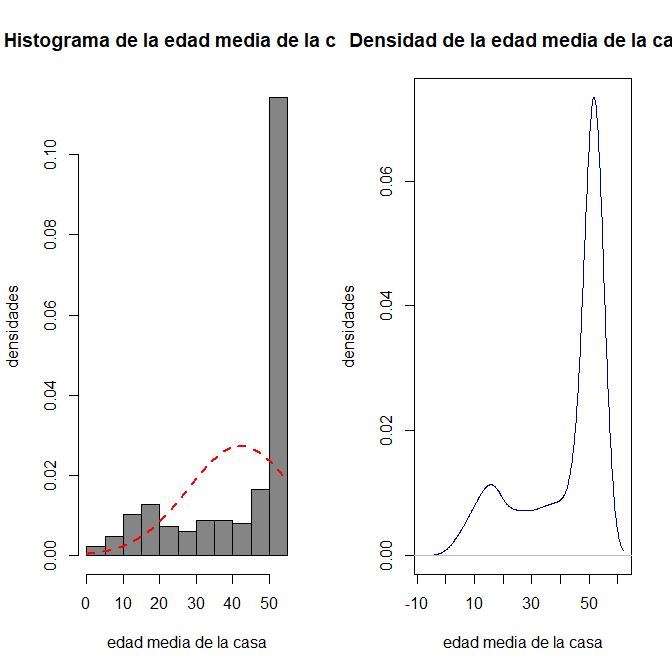
\includegraphics[width=11cm]{imagenes/3.png}
        \caption{Histograma y densidad de la variable 'Edad mediana de las viviendas'}
        \label{fig:Densidad}
    \end{center}
\end{figure}
\end{frame}
\begin{frame}
\frametitle{Variable 'Edad mediana de las viviendas'}
\begin{figure}[!h]
    \begin{center}
        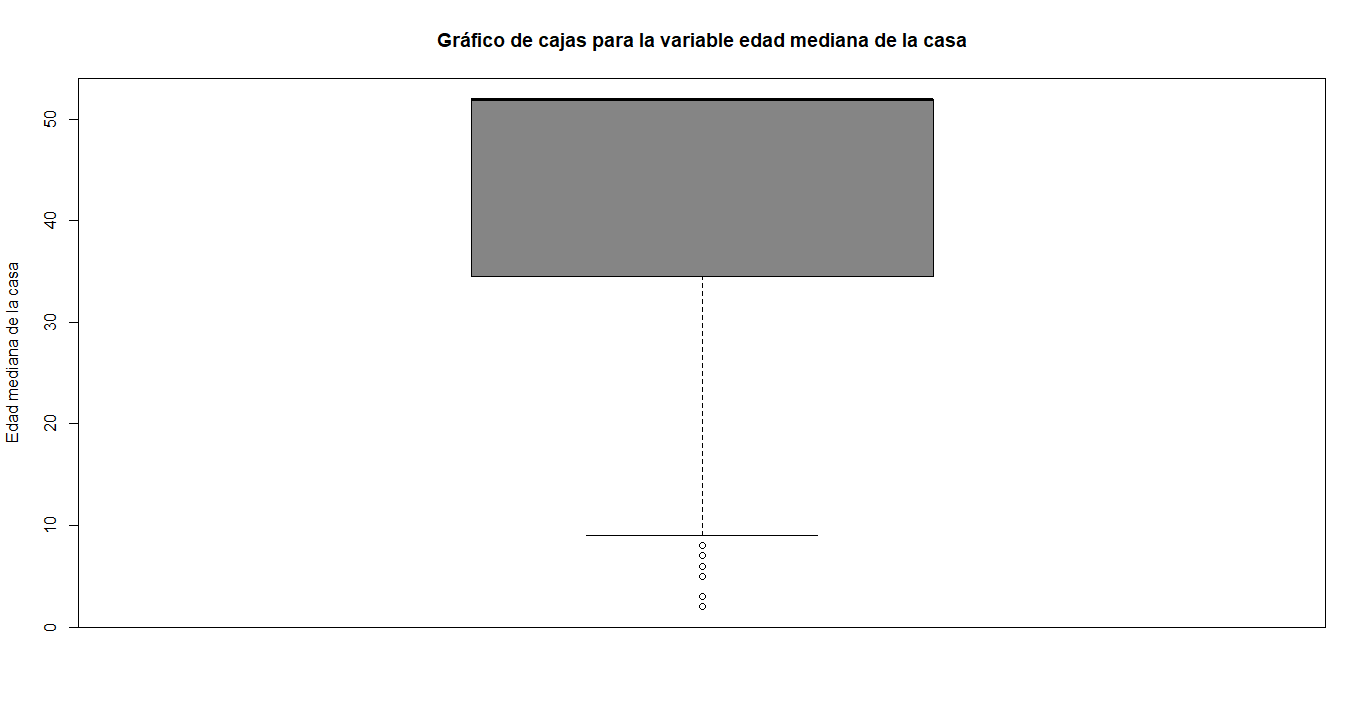
\includegraphics[width=11cm]{imagenes/14.png}
        \caption{Gráfico de cajas para la variable 'Edad mediana de las viviendas'}
        \label{fig:Densidad}
    \end{center}
\end{figure}
\end{frame}

\begin{frame}
\frametitle{Variable 'Total de habitaciones'}
\begin{figure}[!h]
    \begin{center}
        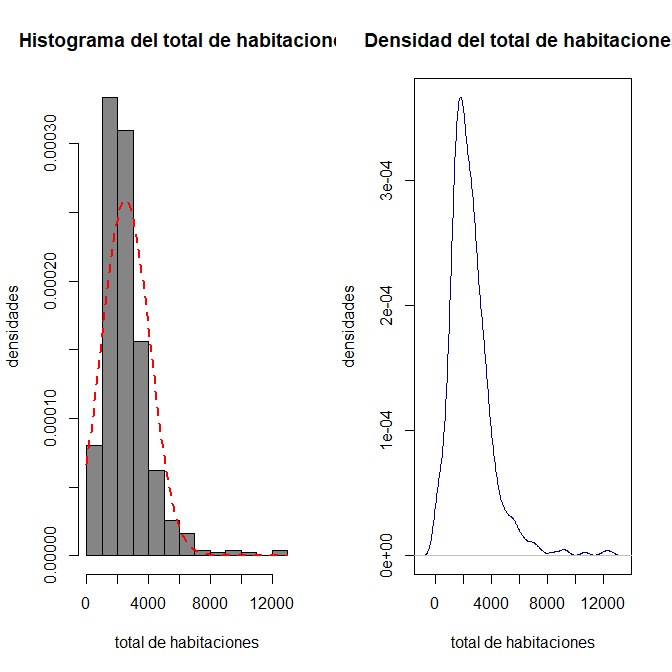
\includegraphics[width=11cm]{imagenes/4.png}
        \caption{Histograma y densidad de la variable 'Total de habitaciones'}
        \label{fig:Densidad}
    \end{center}
\end{figure}
\end{frame}
\begin{frame}
\frametitle{Variable 'Total de habitaciones'}
\begin{figure}[!h]
    \begin{center}
        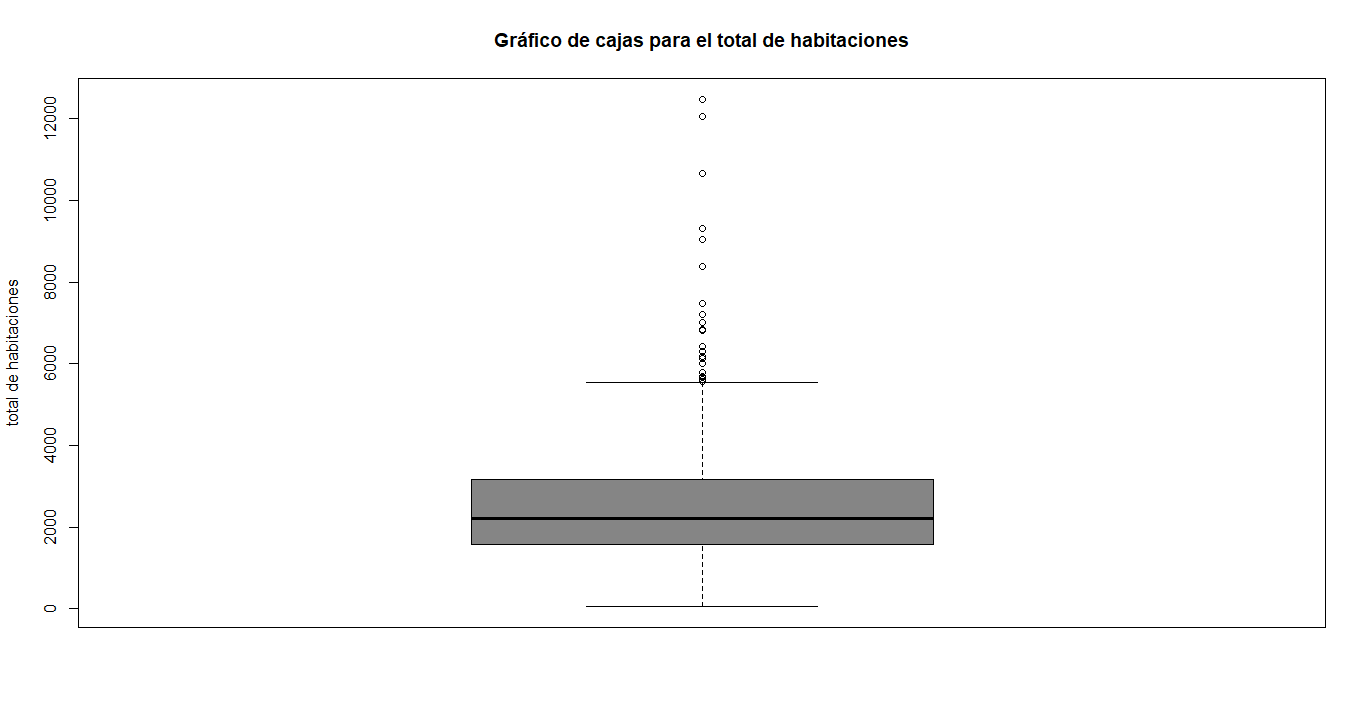
\includegraphics[width=11cm]{imagenes/15.png}
        \caption{Gráfico de cajas para la variable 'Total de habitaciones'}
        \label{fig:Densidad}
    \end{center}
\end{figure}
\end{frame}

\begin{frame}
\frametitle{Variable 'Total de dormitorios'}
\begin{figure}[!h]
    \begin{center}
        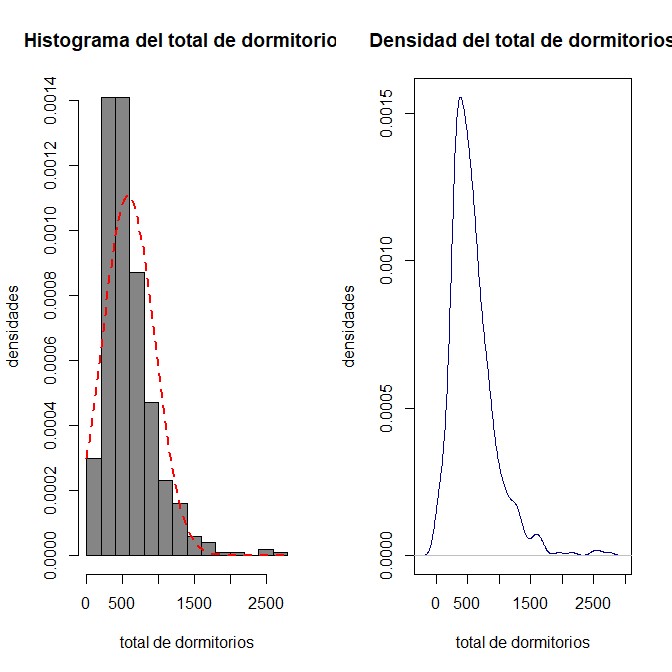
\includegraphics[width=11cm]{imagenes/5.png}
        \caption{Histograma y densidad de la variable 'Total de dormitorios'}
        \label{fig:Densidad}
    \end{center}
\end{figure}
\end{frame}
\begin{frame}
\frametitle{Variable 'Total de dormitorios'}
\begin{figure}[!h]
    \begin{center}
        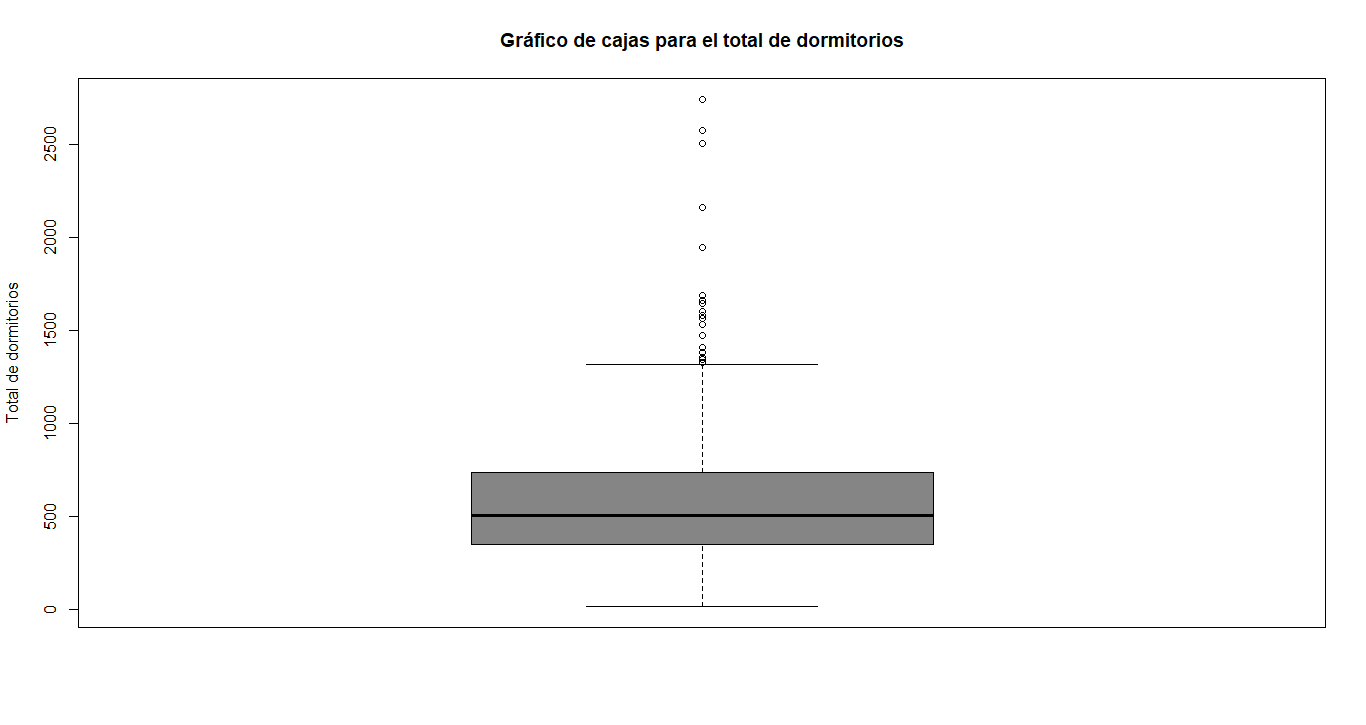
\includegraphics[width=11cm]{imagenes/16.png}
        \caption{Gráfico de cajas para la variable 'Total de dormitorios'}
        \label{fig:Densidad}
    \end{center}
\end{figure}
\end{frame}
\begin{frame}
\frametitle{Variable 'Población'}
\begin{figure}[!h]
    \begin{center}
        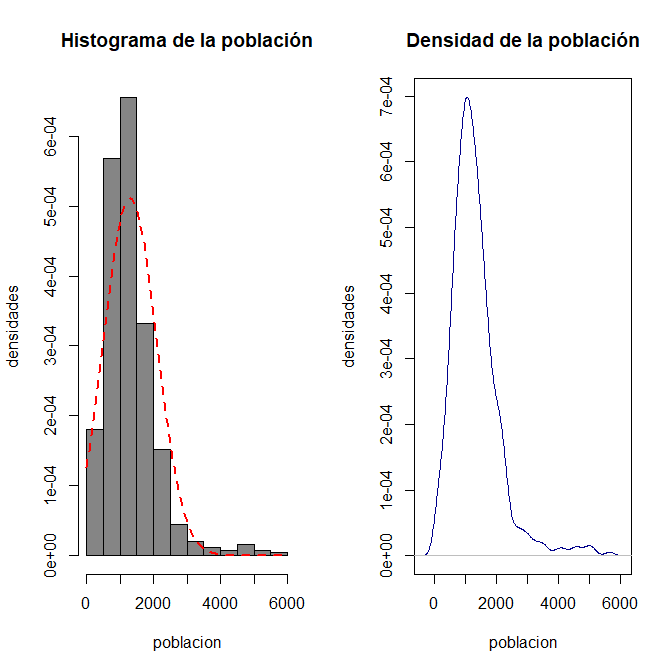
\includegraphics[width=11cm]{imagenes/6.png}
        \caption{Histograma y densidad de la variable 'Población'}
        \label{fig:Densidad}
    \end{center}
\end{figure}
\end{frame}
\begin{frame}
\frametitle{Variable 'Población'}
\begin{figure}[!h]
    \begin{center}
        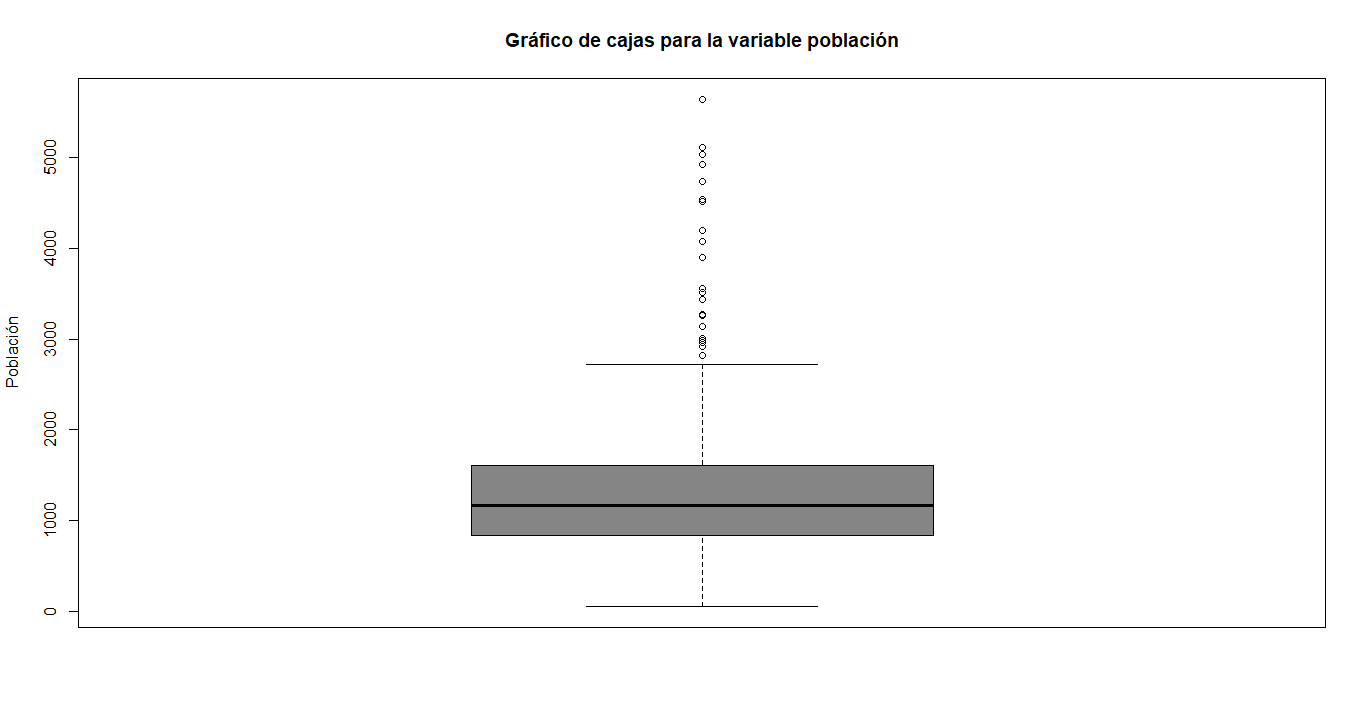
\includegraphics[width=11cm]{imagenes/17.png}
        \caption{Gráfico de cajas para la variable 'Población'}
        \label{fig:Densidad}
    \end{center}
\end{figure}
\end{frame}

\begin{frame}
\frametitle{Variable 'Hogares'}
\begin{figure}[!h]
    \begin{center}
        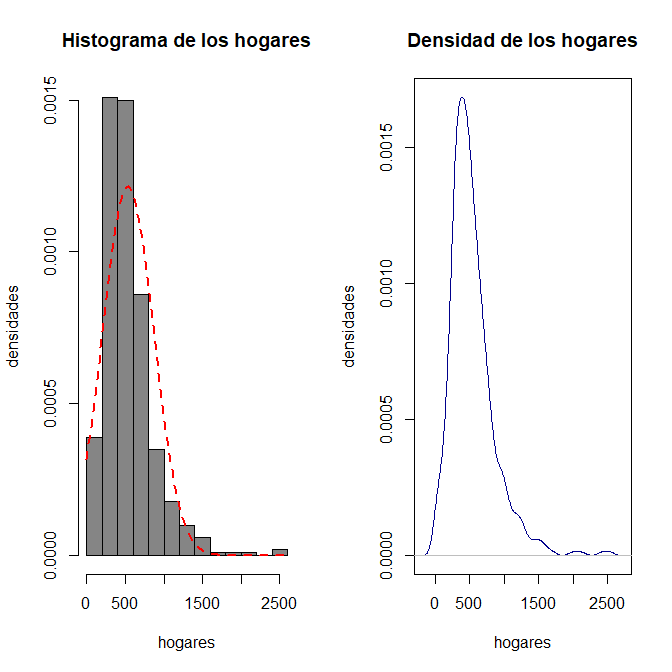
\includegraphics[width=11cm]{imagenes/7.png}
        \caption{Histograma y densidad de la variable 'Hogares'}
        \label{fig:Densidad}
    \end{center}
\end{figure}
\end{frame}
\begin{frame}
\frametitle{Variable 'Hogares'}
\begin{figure}[!h]
    \begin{center}
        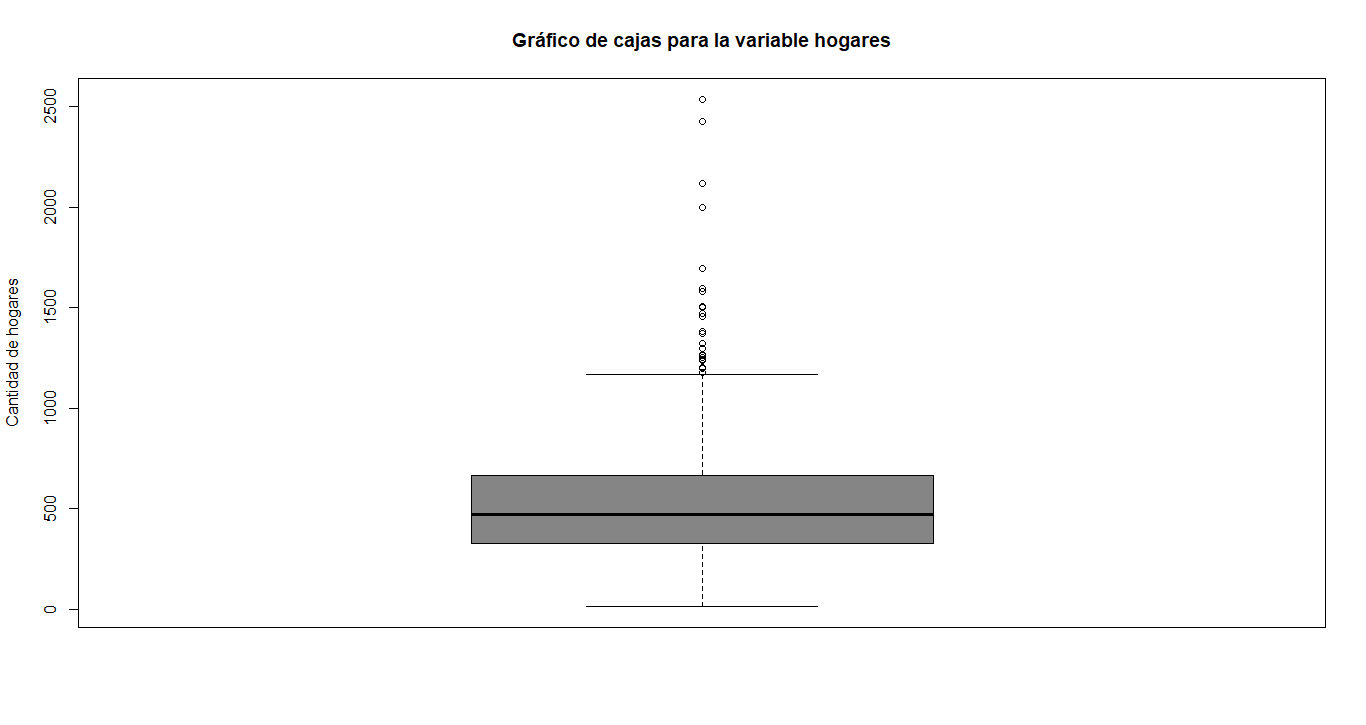
\includegraphics[width=11cm]{imagenes/18.png}
        \caption{Gráfico de cajas para la variable 'Hogares'}
        \label{fig:Densidad}
    \end{center}
\end{figure}
\end{frame}

\begin{frame}
\frametitle{California}
\begin{figure}[!h]
    \begin{center}
        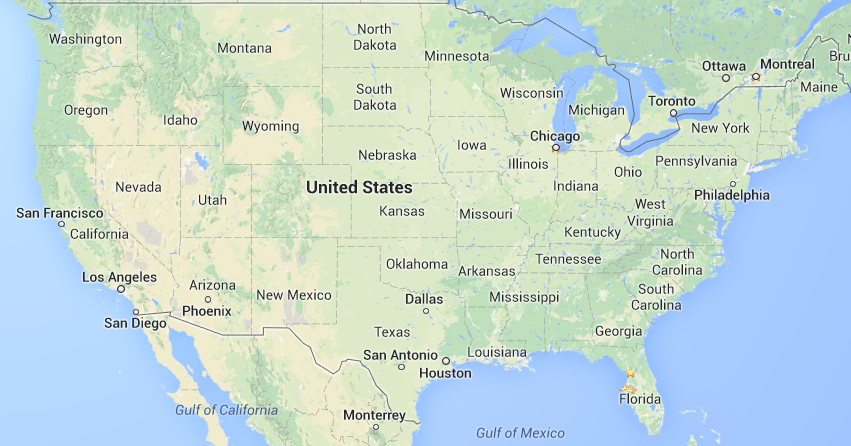
\includegraphics[width=11cm]{imagenes/california.png}
        \caption{Lugar de donde provienen los datos}
        \label{fig:Densidad}
    \end{center}
\end{figure}
\end{frame}

\begin{frame}
\frametitle{San Francisco}
\begin{figure}[!h]
    \begin{center}
        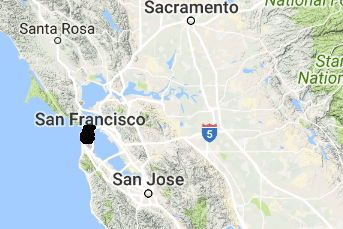
\includegraphics[width=11cm]{imagenes/sanfransisco.png}
        \caption{Mapa con los puntos dados de longitud y latitud}
        \label{fig:Densidad}
    \end{center}
\end{figure}
\end{frame}

\begin{frame}
\frametitle{San Diego}
\begin{figure}[!h]
    \begin{center}
        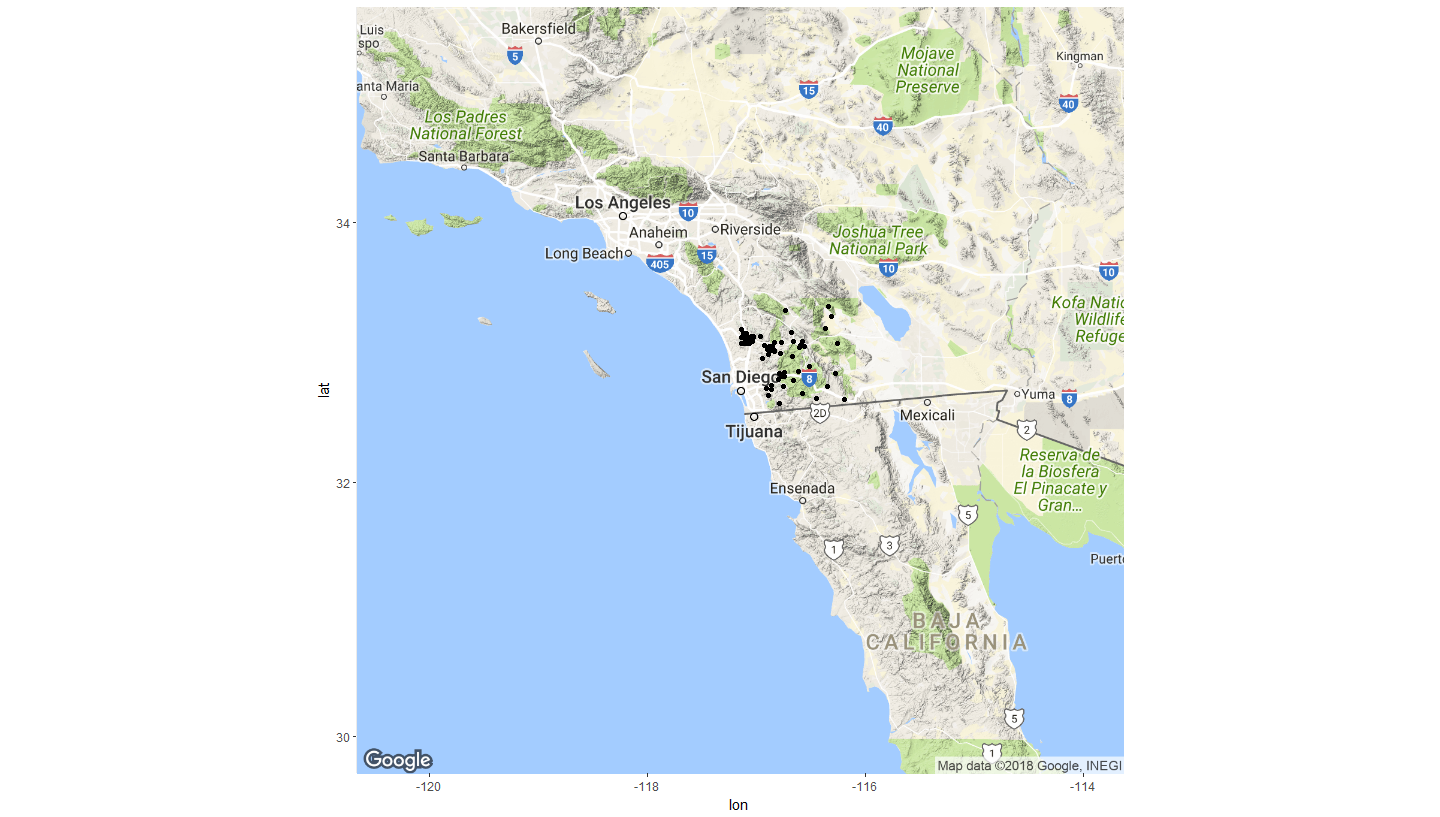
\includegraphics[width=11cm]{imagenes/sandiego.png}
        \caption{Mapa con los puntos dados de longitud y latitud}
        \label{fig:Densidad}
    \end{center}
\end{figure}
\end{frame}

\begin{frame}
\frametitle{Posibles relaciones entre las variables explicativas}
\begin{itemize}
\item Matriz de correlaciones:
\begin{figure}[!h]
       \raggedright
        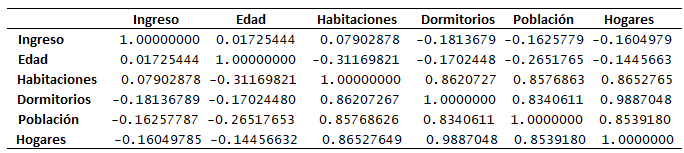
\includegraphics[width=11.2cm]{imagenes/correlacion.png}
        \caption{Matriz de correlaciones entre covariables }
        \label{fig:Densidad}
\end{figure}
\end{itemize}
\end{frame}

\begin{frame}
\frametitle{Posibles relaciones entre las variables explicativas}
\begin{itemize}
\item Variables 'Total de dormitorios' y 'Hogares':
\begin{figure}[!h]
    \begin{center}
        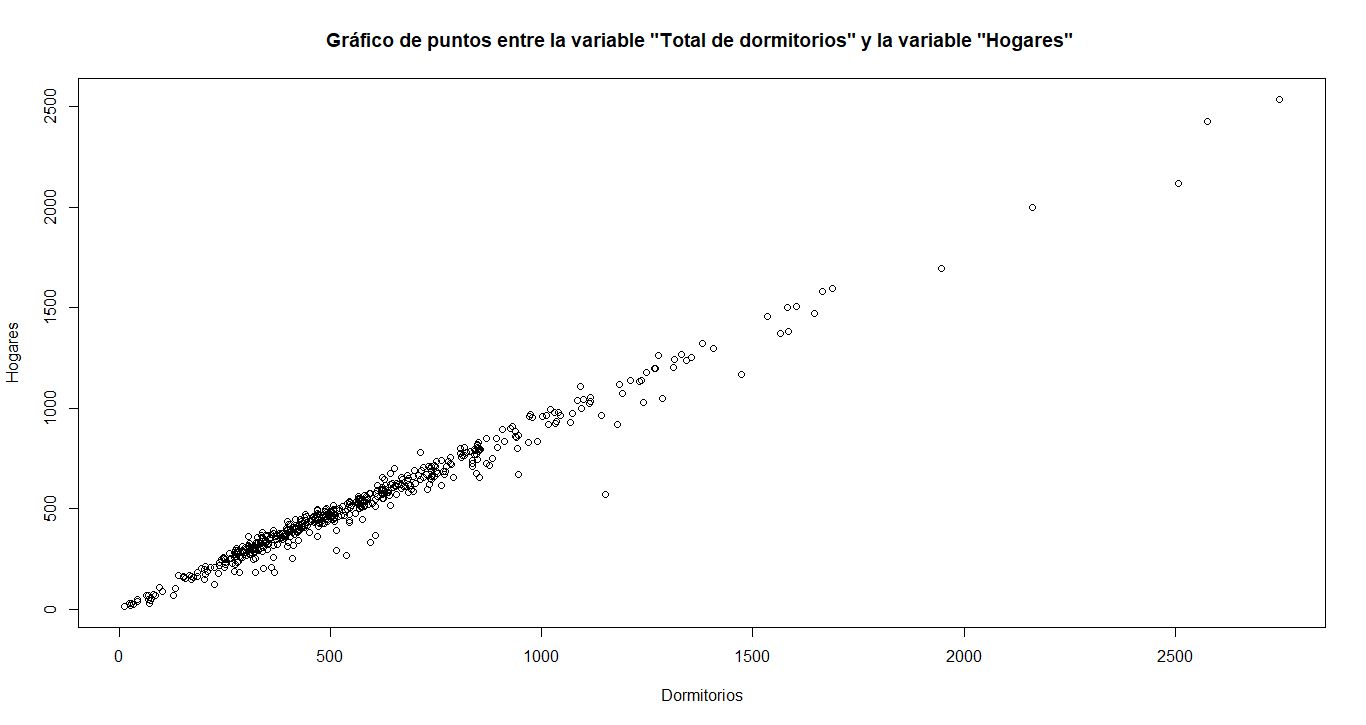
\includegraphics[width=10cm]{imagenes/19.png}
        \caption{Gráfico de puntos entre las variables 'Total de dormitorios' y 'Hogares'}
        \label{fig:Densidad}
    \end{center}
\end{figure}
\end{itemize}
\end{frame}

\begin{frame}
\frametitle{Posibles relaciones entre las variables explicativas}
\begin{itemize}
\item correlación de Pearson: $r=0.9887048$
\item correlación de Spearman: $\rho=0.9819133$
\end{itemize}
\end{frame}

\begin{frame}
\frametitle{Posibles relaciones entre las variables explicativas}
\begin{itemize}
\item Variables 'Población' y 'Hogares':
\begin{figure}[!h]
    \begin{center}
        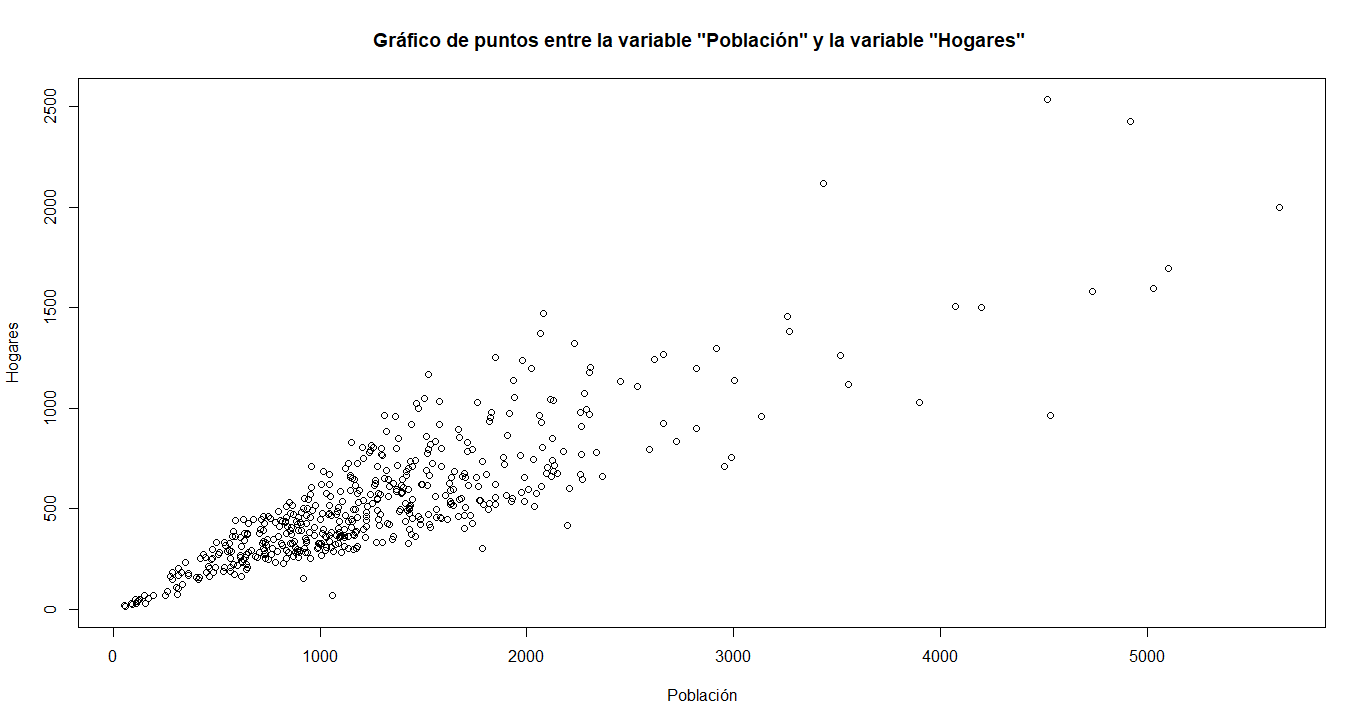
\includegraphics[width=10cm]{imagenes/10.png}
        \caption{Gráfico de puntos entre las variables 'Población' y 'Hogares'}
        \label{fig:Densidad}
    \end{center}
\end{figure}
\end{itemize}
\end{frame}

\begin{frame}
\frametitle{Posibles relaciones entre las variables explicativas}
\begin{itemize}
\item correlación de Pearson: $r=0.853918$
\item correlación de Spearman: $\rho=0.8395669$
\end{itemize}
\end{frame}

\begin{frame}
\frametitle{Posibles relaciones entre las variables explicativas}
\begin{itemize}
\item Variables 'total de habitaciones' y 'total de dormitorios':
\begin{figure}[!h]
    \begin{center}
        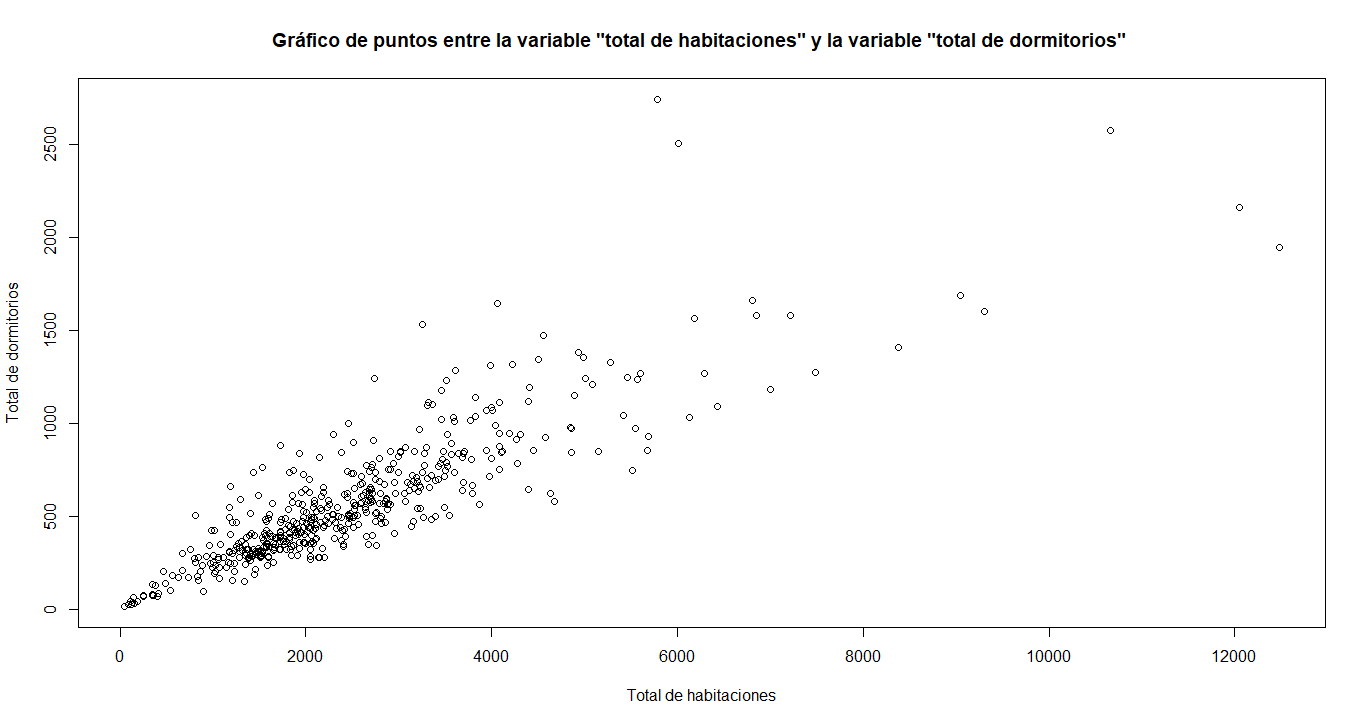
\includegraphics[width=10cm]{imagenes/11.png}
        \caption{Gráfico de puntos entre las variables 'total de habitaciones' y 'total de dormitorios'}
        \label{fig:Densidad}
    \end{center}
\end{figure}
\end{itemize}
\end{frame}

\begin{frame}
\frametitle{Posibles relaciones entre las variables explicativas}
\begin{itemize}
\item correlación de Pearson: $r=0.862072$
\item correlación de Spearman: $\rho=0.8716658$
\end{itemize}
\end{frame}

\begin{frame}
\frametitle{Modelo ajustado e interpretación}
~\\ El modelo ajustado incluyendo todas las variables sin transformación y sin selección de variables es:
~\\ $Y=57720.52+24261.20X_{1}+3443.94X_{2}+19.09X_{3}-67.72X_{4}-121.66X_{5}+315.92X_{6}$

~\\ Donde: Y=Valor mediano de la casa, $X_{1}=$Ingreso mediano, $X_{2}=$Edad mediana de la vivienda, $X_{3}=$Total de habitaciones, $X_{4}=$Total de dormitorios, $X_{5}=$Población, $X_{6}=$Hogares.
\begin{itemize}
\item $R^2=0.5425$
\item $R^2_{ajustado}=0.537$
\item $CME=\hat{\sigma^2}=6724487923$
\end{itemize}
\end{frame}


\begin{frame}
\frametitle{Modelo ajustado e interpretación}
\begin{itemize}
\item $\beta_{0}$:Representa el valor del intercepto con el eje y, esto quiere decir que Y va a partir de un valor de 57720.52 sin importar en cuantas unidades aumente mis otras variables.  
\item $\beta_{1}$:por cada unidad que aumente de ingreso mediano se aumentan 24261.20 unidades del valor mediano de la casa.
\item $\beta_{2}$:por cada unidad que aumente de edad mediana de la vivienda se aumentan 3443.94 unidades del valor mediano de la casa.
\item $\beta_{3}$:por cada unidad que aumente de total de habitaciones se aumentan 19.09 unidades del valor mediano de la casa.
\item $\beta_{4}$:por cada unidad que aumente de total de dormitorios se disminuye 67.72 unidades del valor mediano de la casa.
\end{itemize}
\end{frame}
\begin{frame}
\begin{itemize}
\item $\beta_{5}$:por cada unidad que aumente de población se disminuye 121.66 unidades del valor mediano de la casa.
\item $\beta_{6}$:por cada unidad que aumente de hogares se aumenta 315.92 unidades del valor mediano de la casa.
\end{itemize}
\end{frame}

\begin{frame}
\frametitle{Modelo ajustado con selección de variables}
~\\ El modelo ajustado, utilizando el método forward para seleccionar variables es exactamente el mismo modelo completo, es decir, el método no me elimino ninguna variable.
\end{frame}

\begin{frame}
\frametitle{Modelo ajustado con selección de variables}
~\\ El modelo ajustado, utilizando el método backward para seleccionar variables es:
~\\ $Y=52921.688+24923.244X_{1}+3484.164X_{2}+17.588X_{3}-118.652X_{5}+243.265X_{6}$

~\\ Donde: Y=Valor mediano de la casa, $X_{1}=$Ingreso mediano, $X_{2}=$Edad mediana de la vivienda, $X_{3}=$Total de habitaciones, $X_{5}=$Población, $X_{6}=$Hogares.
\begin{itemize}
\item $R^2=0.5417$
\item $R^2_{ajustado}=0.5371$
\item $CME=\hat{\sigma^2}=6722361839$
\end{itemize}
\end{frame}

\begin{frame}
\frametitle{Modelo ajustado con selección de variables}
~\\ El modelo ajustado, utilizando el método stepwise para seleccionar variables es  exactamente el mismo modelo que ajustamos por el método anterior (backward), es decir, ambos métodos nos eliminan la variable $X_{4}=$Total de dormitorios del modelo completo.
\end{frame}

\begin{frame}
\frametitle{Comparación}
\begin{figure}[!h]
    \begin{center}
        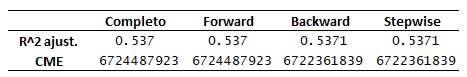
\includegraphics[width=11cm]{imagenes/comparacion.png}
        \caption{Comparación de los modelos generados con selección de variables}
        \label{fig:Densidad}
    \end{center}
\end{figure}
\end{frame}

\begin{frame}
\frametitle{Conclusión}
~\\ Al finalizar nuestra selección de variables, con el fin de ajustar el mejor modelo posible para la variable valor mediano de la casa, comparamos cada uno de los 4 modelos obtenidos (completo, forward, backward, stepwise) con respecto al $R^2_{ajustado}$ y el $CME=\hat{\sigma^2}$. Podemos concluir que el mejor modelo que logramos obtener  para nuestros 500 datos sin hacer transformación de variables, fue el generado por el método de selección 'Backward'      y 'Stepwise', los cuales nos eliminaron la variable explicativa $X_{4}:$Total de dormitorios.
\end{frame}

\end{document}